\documentclass{article}
\usepackage{url}
\usepackage{mathtools}
\usepackage{amsmath}
\usepackage{listings}
\usepackage{graphicx}
\usepackage[margin=1in]{geometry}
\usepackage{float}
\lstset{breaklines=true}
\begin{document}

\title{CS595 Intro to Web Science, Assignment \#1}
\author{Valentina Neblitt-Jones}
\date{September 12, 2013}
\maketitle

\section{cURL Exercise}
\textbf {Demonstrate that you know how to use "curl" well enough to correctly POST data to a form.  Show that the HTML response that is returned is "correct" (e.g., save it to a file and then view that file in a browser and take a screen shot).}

Finding a web form that did not require me revealing my credentials and actually used the POST method was quite difficult. I used W3C Markup Validator Service \url{http://validator.w3.org/#validate_by_input}. It was being extra fussy about the special characters (--urlencode was not solving the problem) so so I had to substitute the appropriate URL encoding using \url{http://www.w3schools.com/tags/ref_urlencode.asp}. My cURL statement follows.

\begin{lstlisting}
curl --data "fragment=%3Cp%3ECurrently I am 40 years old and an academic systems librarian. My passions are books, movies, and television. My ultra-passions include Star Wars, LEGO, The Simpsons, and Harry Potter.%3C%2Fp%3E&prefill=1&doctype=Inline&fbd=1&prefill_doctype=html401&group=0&ss=1&st=1&outline=1&No200=1&verbose=1" --url http://validator.w3.org/check -o debug.html
\end{lstlisting}

The four screenshots below illustrate the difference in how the page was rendered when using the browser versus cURL to fill out the form. Figures 1 \& 2 show the browser version and Figures 3 \& 4 show the cURL version. Although the stylesheet and images are missing from the cURL version, the same information is present.

\begin{figure}[H]
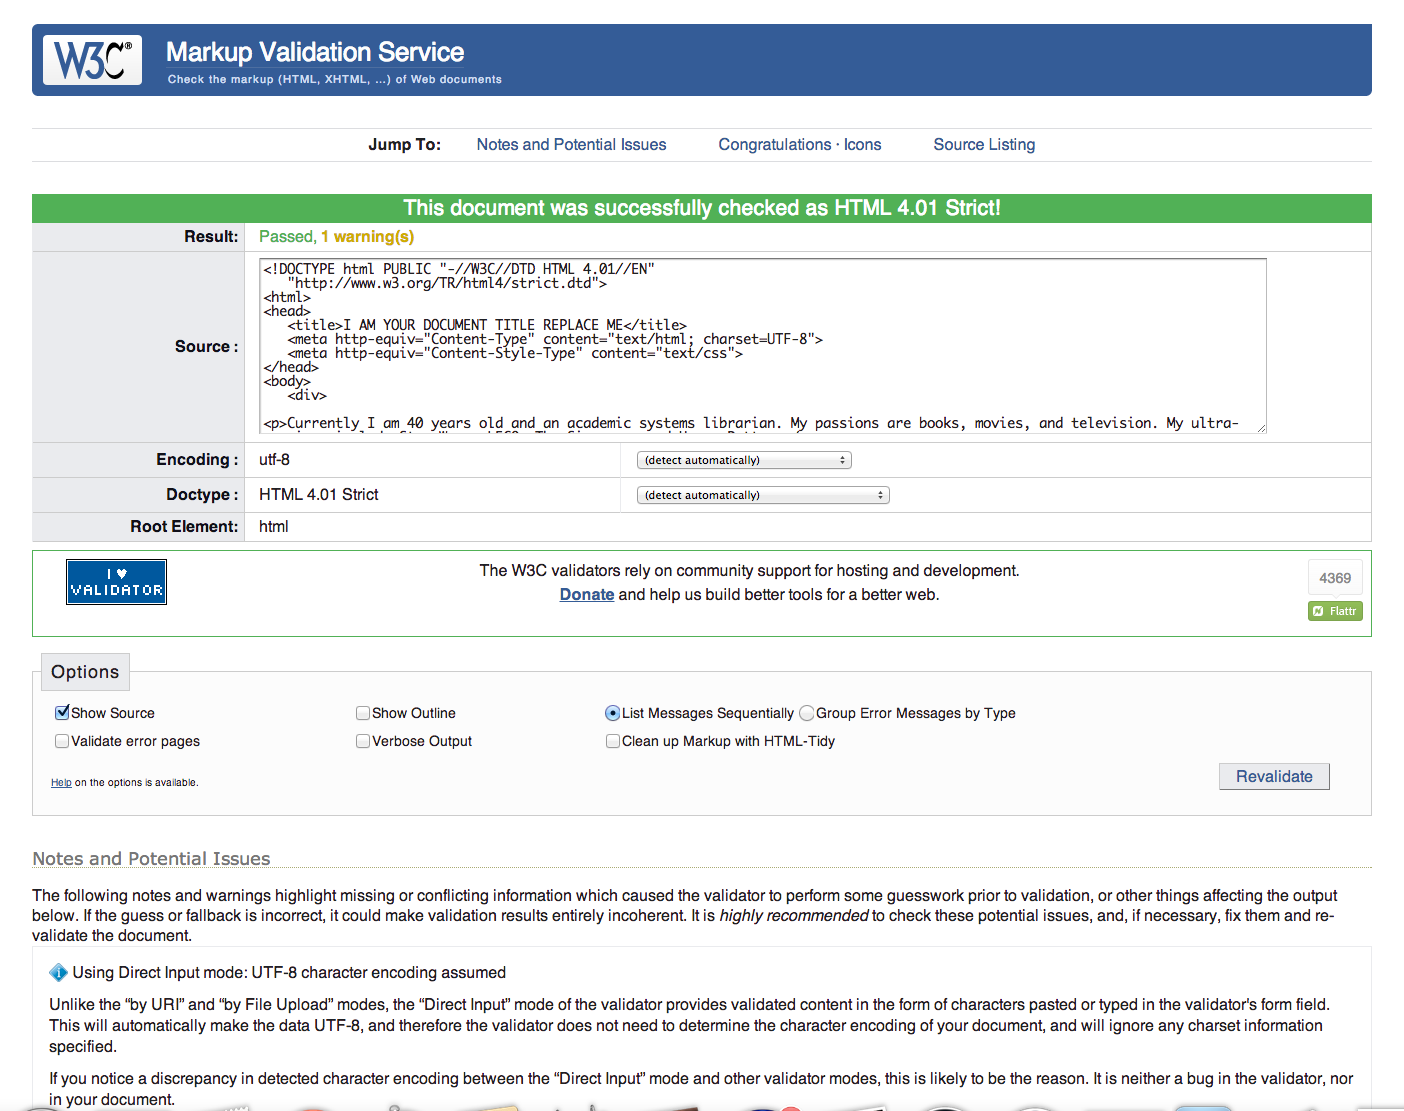
\includegraphics[scale=0.30]{w3cMarkupValidationServiceNormal01}
\caption{This is the top half of the screen representing output when the browser was used to fill out the form}
\end{figure}

\begin{figure}[H]
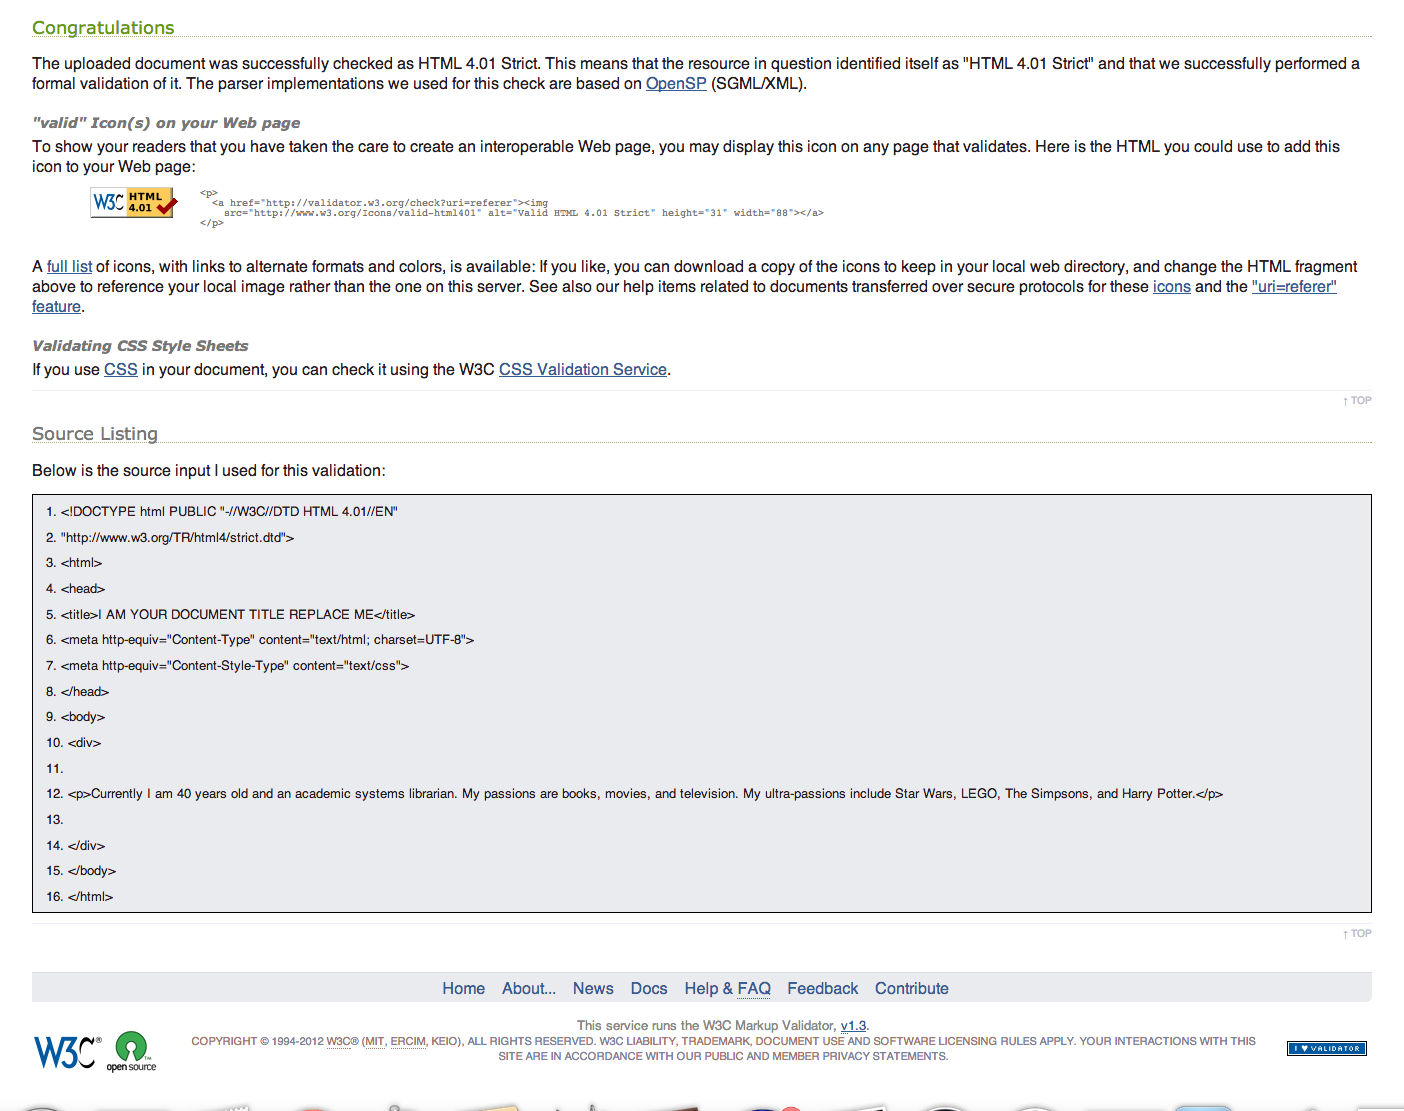
\includegraphics[scale=0.30]{w3cMarkupValidationServiceNormal02}
\caption{This is the bottom half of the screen representing output when the browser was used to fill out the form}
\end{figure}

\begin{figure}[H]
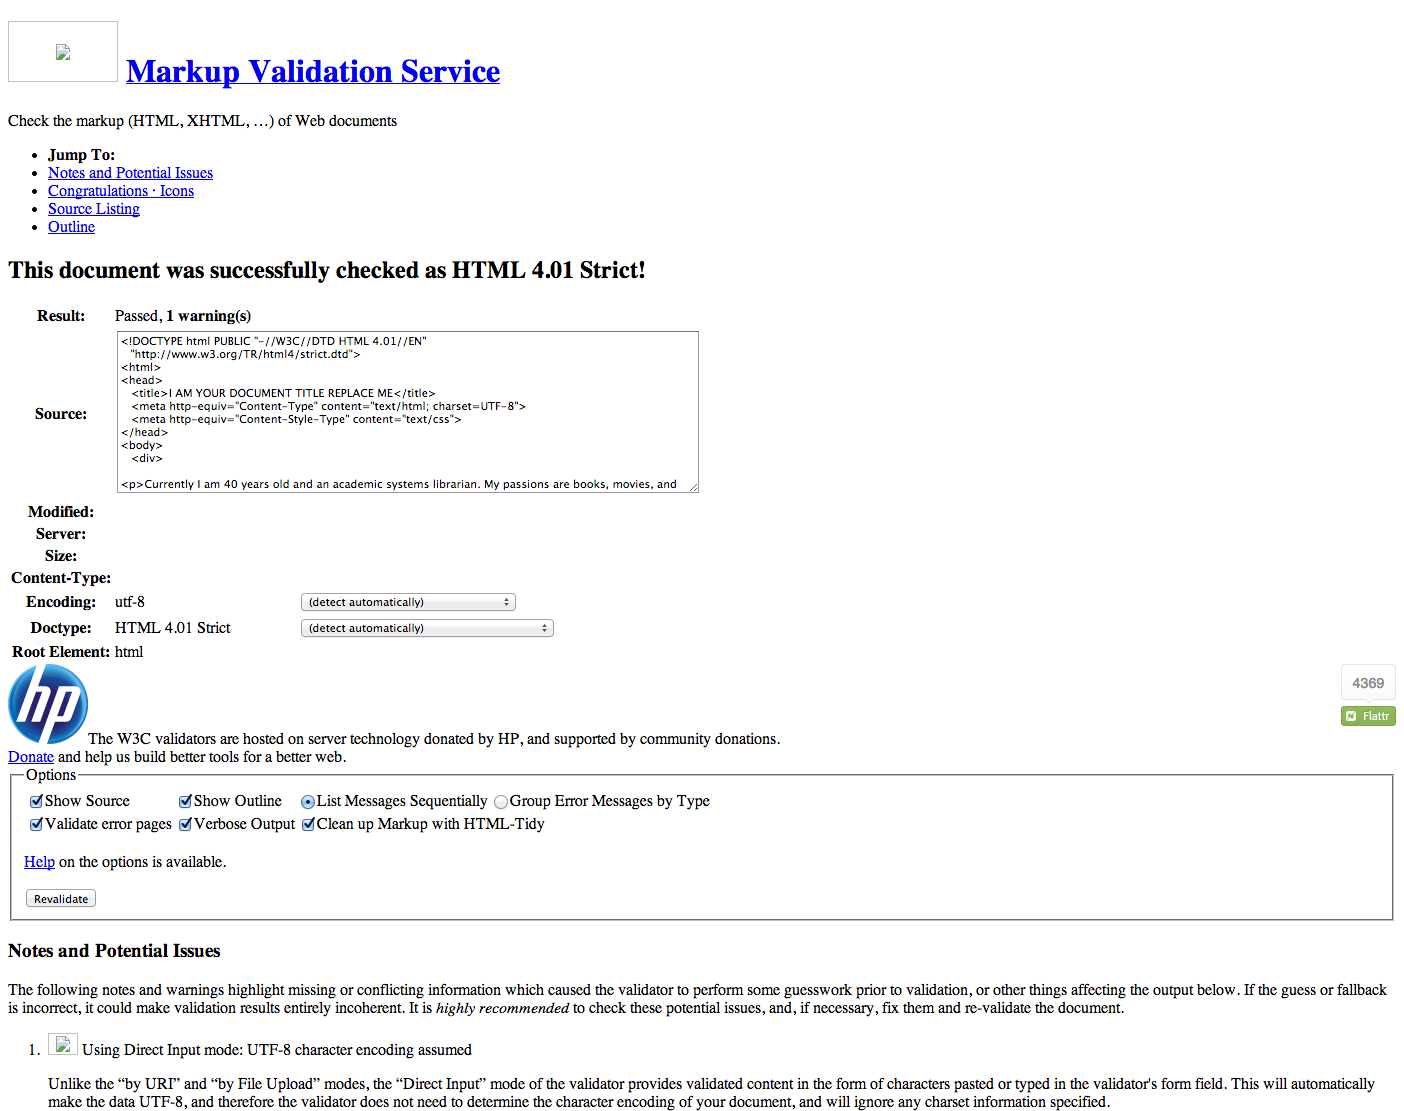
\includegraphics[scale=0.30]{w3cMarkupValidationServiceCurl01}
\caption{This is the top half of the screen representing output when cURL was used to fill out the form}
\end{figure}

\begin{figure}[H]
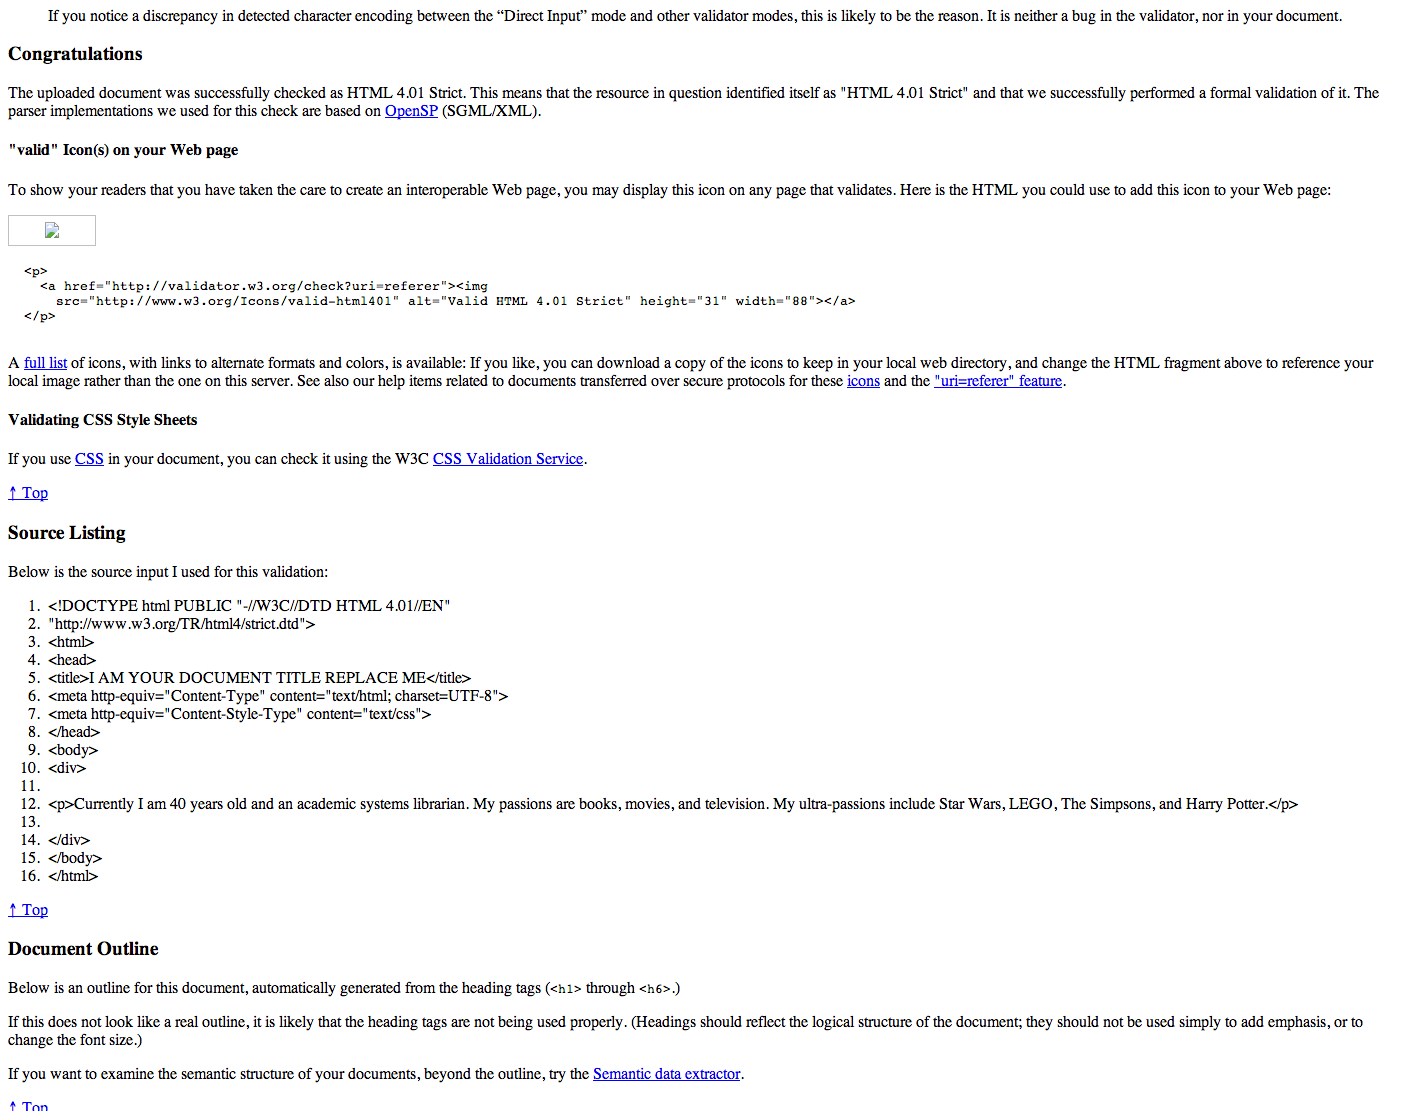
\includegraphics[scale=0.30]{w3cMarkupValidationServiceCurl02}
\caption{This is the bottom half of the screen representing output when cURL was used to fill out the form}
\end{figure}

\newpage

\section{Python Exercise}
\textbf{Write a Python program that:
(1)Takes one argument, like "Old Dominion" or "Virginia Tech" (2) takes another argument specified in seconds (e.g., "60" for one minute) (3) takes a URI as a third argument: \url{http://scores.espn.go.com/ncf/scoreboard?confId=80&seasonYear=2013&seasonType=2&weekNumber=2} \textbf{OR} \url{http://scores.espn.go.com/ncf/scoreboard?confId=80&seasonYear=2013&seasonType=2&weekNumber=1} \textbf{OR} \url{http://scores.espn.go.com/ncf/scoreboard?confId=80&seasonYear=2012&seasonType=2&weekNumber=1} etc. and (4) downloads the URI, finds the game corresponding to the team argument, prints out the current score (e.g., "Old Dominion 27, East Carolina 17), sleeps for the specified seconds, and then repeats (until control-C is hit).} 


\subsection*{The Code}

I used Beautiful Soup for this exercise since it was highly advised by classmates. I also needed to use specifically urllib.request since I was using Python 3.3.2. The sys library was used for support accepting arguments from the command line and time was used to support the "sleep" requirement. See Figure 5 for libraries. I used a curl command to capture a live page and use it for testing, but when the code was ready I changed from using the static file to using the live page (Fig. 6). Using "Inspect Element" on Chrome or Firebug on Firefox, I reviewed the page source for the web page and identified tags and attributes containing the pertinent information. Mod-Content (Fig. 7) was the smallest element that contained all the relevant information. Within Mod-Content, Team Visitor and Score classes and Team Home and Score classes held the team name and score (Figs. 8 and 9). I had to run through the <li> tags to find the last score and that method allowed for finding the score even if the game was not over. Once all the information was identified and could be referenced, I was able to create the print statement to output the team names and scores and the statement to time out after the specified seconds in the second argument (Fig. 10). The while statement in Figure 6 was used to make the program continue to look for and output the current score.

\begin{figure}[H]
\centering
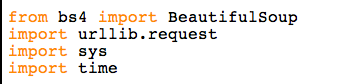
\includegraphics[scale=0.50]{libraries}
\caption{Libraries Used for Exercise}
\end{figure}

\begin{figure}[H]
\centering
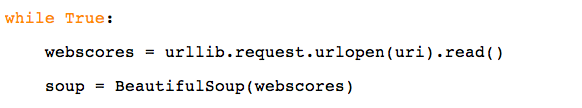
\includegraphics[scale=0.50]{getpageandloop}
\caption{Fetching the web page}
\end{figure}

\begin{figure}[H]
\centering
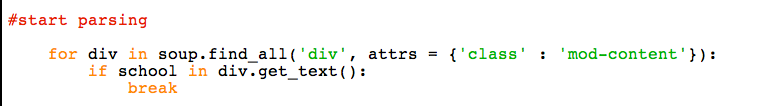
\includegraphics[scale=0.50]{startparsing}
\caption{Libraries Used for Exercise}
\end{figure}

\begin{figure}[H]
\centering
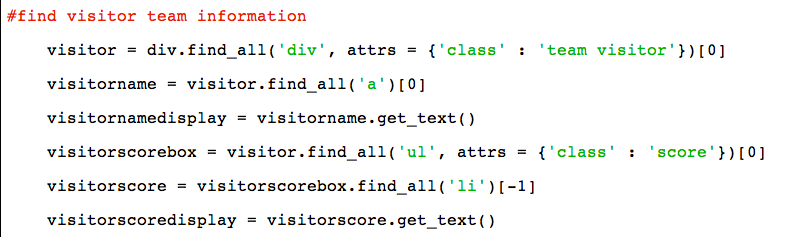
\includegraphics[scale=0.40]{findvisitorteaminfo}
\caption{Code segment for Collecting Visitor Team Information}
\end{figure}

\begin{figure}[H]
\centering
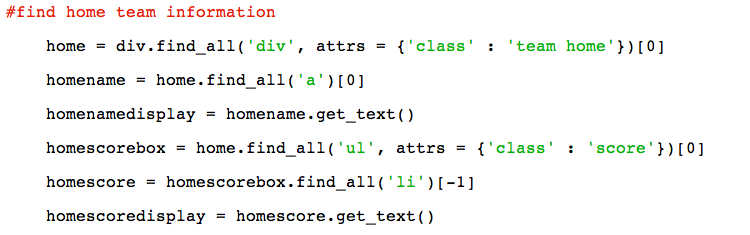
\includegraphics[scale=0.40]{findhometeaminfo}
\caption{Code segment for for Collecting Home Team Information}
\end{figure}

\begin{figure}[H]
\centering
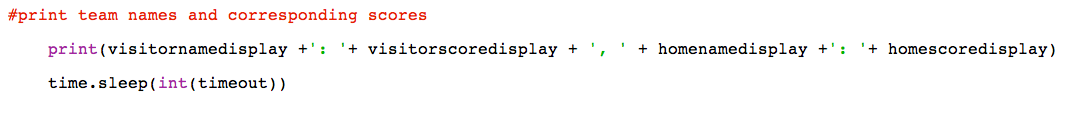
\includegraphics[scale=0.40]{printandend}
\caption{Code segment for Final Output and Time Out}
\end{figure}

\subsection*{The Execution}

Figure 11 shows the execution of the code. The arguments were:

\begin{enumerate}
\item school = Troy
\item timeout = 10
\item uri = \url"http://scores.espn.go.com/ncf/scoreboard?confId=80&seasonYear=2013&seasonType=2&weekNumber=3"
\end{enumerate}

I ran the program during a game that had not finished to test that it would reflect score changes. You can see in the last line that Troy went from 0 to 6 points. You can also see that the program terminates after using Ctrl-C.

\begin{figure}[H]
\centering
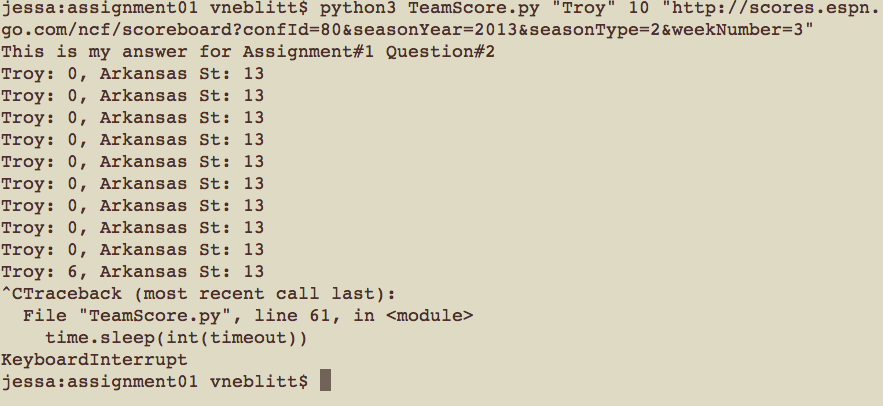
\includegraphics[scale=0.40]{endingOutput}
\caption{Running the Program}
\end{figure}

\subsection*{Further Work}
It seems like I should have been able to have some functions in here so maybe the code is not as elegant as it could be. Furthermore, it does not handle the situation where the "school" is not found on the page well. I had to remind the cataloger in me that the exercise's intention was to learn how to scrape a web page when I desperately wanted to institute name authority control. Name authority control would have taken care of the ODU v. Old Dominion v. Old Dominion University input problem. However, a cursory calculation of the number of schools represented revealed at least 120 schools potentially needing name authority control.


\newpage

\section{Web Graph Structure Exercise}
\textbf{Consider the "bow-tie" graph in the Broder et al. paper (fig 9): \url{http://www9.org/w9cdrom/160/160.html}
Now consider the following graph:}

\begin{verbatim}
A --> B
B --> C
C --> D
C --> A
C --> G
E --> F
G --> C
G --> H
I --> H
I --> J
I --> K
J --> D 
L --> D
M --> A
M --> N
N --> D
\end{verbatim}

\textbf{For the graph above, give the values for: IN, SCC, OUT, Tendrils, Tubes, and Disconnected.}

\newpage

\begin{itemize}
\item IN:
\item SCC:
\item OUT:
\item Tendrils:
\item Tubes:
\item Disconnected: E, F
\end{itemize}


\begin{figure}[H]
\centering
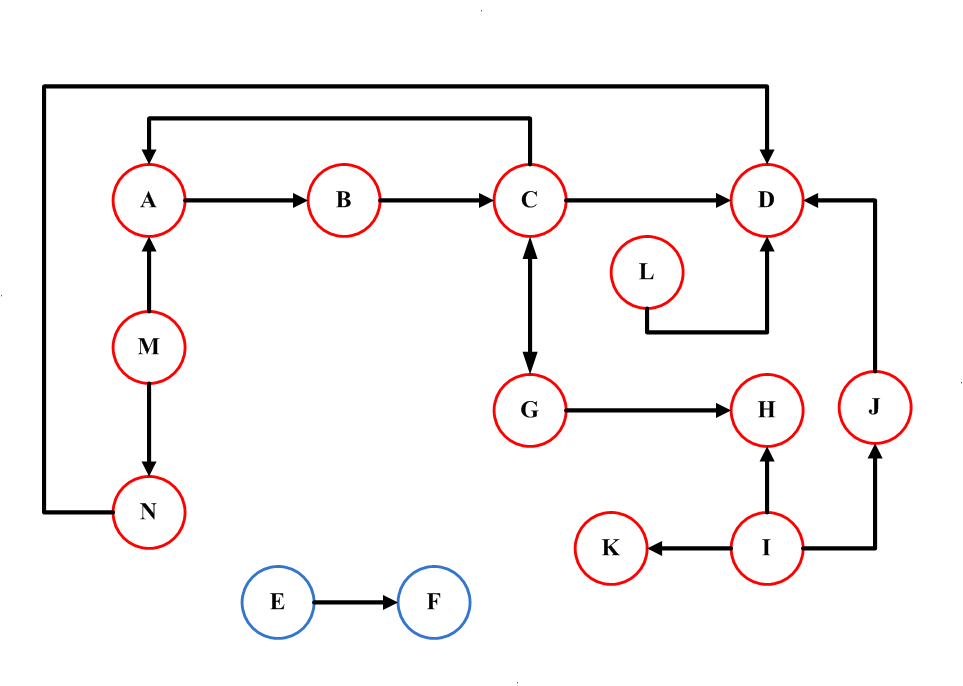
\includegraphics[scale=0.50]{assn01Q03}
\caption{Visual representation of the connecting nodes}
\end{figure}

\end{document}